\documentclass[14pt, openany, titlepage]{report} % Explicitly use openany and titlepage
\usepackage[utf8]{inputenc}
\usepackage[italian,english]{babel}
\usepackage{graphicx}
\usepackage{cite}
\usepackage{amsmath}
\usepackage[table,xcdraw]{xcolor}
\usepackage[italian]{minitoc}
\usepackage{fancybox}
\usepackage{fancyhdr}
\usepackage{verbatim}
\usepackage{url}
\usepackage{color}
\usepackage{listings}
\usepackage{makeidx}
\usepackage{comment}
\usepackage{hyperref}
\usepackage{bm}
\usepackage{longtable}
\usepackage{tabularx}
\usepackage{placeins}
\usepackage{caption}
\usepackage{float}
\usepackage{xcolor}
\usepackage{soul}
\usepackage{array}
\usepackage{multirow}
\usepackage{adjustbox} % Pacchetto per ridimensionare automaticamente
\usepackage{graphicx} % Per il ridimensionamento
\usepackage{lscape}
\usepackage{mathtools}
\usepackage{amsmath}
\usepackage{amssymb}
\usepackage{listings}
\usepackage[svgnames]{xcolor}
\usepackage{booktabs}

% Set link colors without borders
\hypersetup{
    colorlinks=true,
    linkcolor=black,
    filecolor=magenta,      
    urlcolor=cyan,
}

\lstset{frame=tb,
    language=Java,
    numbers=left,
    keywordstyle=\color{blue},
    alsoletter={.}
}

\lstset{language=R,
    basicstyle=\small\ttfamily,
    stringstyle=\color{DarkGreen},
    otherkeywords={0,1,2,3,4,5,6,7,8,9},
    morekeywords={TRUE,FALSE},
    deletekeywords={data,frame,length,as,character},
    keywordstyle=\color{blue},
    commentstyle=\color{DarkGreen},
}

\graphicspath{ {./Figure/} }


% Minimize additional blank pages
\let\cleardoublepage\clearpage % Suppresses new page on odd side
\flushbottom % Avoid vertical blank space between paragraphs

% Title Page
\begin{document}
\selectlanguage{italian}

\begin{titlepage}
\begin{center}
    \begin{figure}
        
\includegraphics[width=3.5cm, height=3.5cm]{unisa.png}
        \centering
    \end{figure}
    {\Large Università degli Studi di Salerno}\\[0.2truecm]
    {\large Dipartimento di Informatica\\Corso di Laurea Triennale in Informatica}\\
    \hrulefill
    \vfill
    {\large Progetto Calcolo Probabilità Statistica Matematica\\(CPSM)}\\[0.1truecm]
    \vfill\vfill
    {\LARGE {\bf Indagine Statistica sulle\\[0.1truecm]Morti in incidenti stradali}}
    \vfill\vfill
    
    \hfill  \textbf{Tozza Gennaro Carmine}
    \centerline{\hfill Matricola: 0512120382}
    
    \vfill
    \hrulefill 
    \begin{center} Anno Accademico 2024-2025 \end{center}
\end{center}
\end{titlepage}

% Suppress page break after table of contents
\tableofcontents

\chapter{Introduzione}
\section{Problematica}
Gli \textbf{incidenti stradali} costituiscono una delle principali emergenze 
di sanità pubblica, in quanto responsabili ogni anno di un elevato 
numero di decessi, in particolare tra i giovani, e di gravi conseguenze
 in termini di disabilità temporanee e permanenti, oltre al drammatico impatto umano e psicologico sulle vittime e 
 sulle loro famiglie. 
\noindent

\section{Scopo del progetto}
Il progetto consiste in un’indagine statistica \footnote{\url{https://siqual.istat.it/SIQual/visualizza.do?id=7777778&refresh=true&language=IT}}sugli incidenti stradali verificatisi sulla rete stradale del territorio nazionale, tra il 2010 e il 2023 verbalizzati da un'autorità di Polizia o dai Carabinieri, 
avvenuti su una strada aperta alla circolazione pubblica e che hanno causato lesioni a persone, morti (entro il 30° giorno) e/o feriti, con il coinvolgimento 
di almeno un veicolo. \\\\
\noindent
La rilevazione è condotta correntemente dall’Istat, con la compartecipazione dell'ACI e di numerosi Enti pubblici istituzionali, 
è a carattere totale e a cadenza mensile (inserita tra le rilevazioni di interesse pubblico nel Programma Statistico Nazionale - PSN - IST00142). \\\\
\noindent
Per l'analisi dei dati è stato scelto l'ambiente di calcolo statistico \textbf{R}. \\
R fornisce un'ampia varietà di tecniche statistiche (modellazione lineare e non lineare, test statistici classici, analisi delle serie temporali, classificazione, \dots)
e grafiche ed è altamente estensibile.\\\\
\noindent
Uno dei punti di forza di R è la facilità con cui possono essere prodotti grafici ben progettati e di qualità per la pubblicazione, 
compresi simboli matematici e formule se necessario.\\\\
\noindent
Per semplificare l'analisi, si è scelto di lavorare non sull'intero dataset, 
ma su un sottoinsieme filtrato di dati, relativo alle morti per incidenti stradali che riguardano solo i conducenti di età compresa tra i 21 e i 24 anni.\\\\
\noindent
Per approfondire l'analisi con dati dettagliati e specifici, è possibile consultare il dataset direttamente sul sito dell'ISTAT al seguente link:
\url{https://esploradati.istat.it/databrowser/#/it/dw/categories/IT1,Z0810HEA,1.0/HEA_ROAD/IT1,41_270_DF_DCIS_MORTIFERITISTR1_1,1.0}\\\\
\noindent
Il dataset in formato CSV è stato ottenuto dalla fonte ISTAT tramite il link indicato, assicurando così l'affidabilità dei dati.\\
Il formato scelto (CSV) permette un'agevole manipolazione dei dati, essendo compatibile con la maggior parte dei software statistici e
dei fogli di calcolo, ottimizzando l'analisi e la visualizzazione delle informazioni.\\\\

\begin{table}[h]
\centering
\begin{minipage}{\linewidth} 
\footnotesize
\centering
\scalebox{0.9}{ % Riduzione leggera
\begin{tabular}{@{}lrrrrrrrrrrrrrr@{}}
\toprule
\textbf{Intersezione} & \textbf{'10} & \textbf{'11} & \textbf{'12} & \textbf{'13} & \textbf{'14} & \textbf{'15} & \textbf{'16} & \textbf{'17} & \textbf{'18} & \textbf{'19} & \textbf{'20} & \textbf{'21} & \textbf{'22} & \textbf{'23} \\
\midrule
Incrocio & 55 & 45 & 42 & 23 & 34 & 24 & 28 & 25 & 23 & 13 & 15 & 16 & 21 & 10 \\
Rotatoria & 7 & 4 & 2 & 5 & 5 & 1 & 5 & 3 & 1 & 2 & 1 & 2 & -- & 3 \\
Rettilineo & 92 & 102 & 89 & 82 & 96 & 95 & 66 & 70 & 60 & 72 & 66 & 69 & 69 & 74 \\
Curva & 58 & 51 & 48 & 46 & 45 & 44 & 41 & 36 & 38 & 42 & 23 & 40 & 27 & 38 \\
Dosso/Pend. & 2 & 7 & 2 & 4 & 2 & 3 & 5 & 1 & 2 & 3 & 2 & 4 & 3 & 1 \\
Galleria & 1 & 1 & 1 & 1 & -- & 1 & 1 & 1 & -- & -- & 3 & 1 & -- & -- \\
\midrule
\textbf{Tot.} & 215 & 210 & 184 & 161 & 182 & 168 & 146 & 136 & 124 & 132 & 110 & 132 & 120 & 126 \\
\bottomrule
\end{tabular}%
}
\end{minipage}
\end{table}

\normalsize


\chapter{Tabelle delle frequenze}

\begin{center}
\begin{lstlisting}[breaklines=true]
# inclusione librerie
library("tidyverse")
require("tidyverse")
library("dplyr")

# viene caricato il dataset
dati <- read.csv("dati_istat.csv")

# filtraggio dati
dati <- dati %>% select(Intersezione, TIME_PERIOD, Osservazione) 
dati <- dati %>% 
  filter(Intersezione != "Totale") 

# 1. Frequenze assolute per intersezione dell'incidente
freq_assolute <- aggregate(Osservazione ~ Intersezione, data=dati, sum)
colnames(freq_assolute) <- c("Intersezione", "Frequenza_Assoluta")
print(freq_assolute)

# 2. Frequenze relative per intersezione dell'incidente
totale <- sum(freq_assolute$Frequenza_Assoluta)
freq_assolute$Frequenza_Relativa <- freq_assolute$Frequenza_Assoluta / totale
print(freq_assolute)

# 3. Frequenze cumulate assolute
freq_assolute <- freq_assolute[order(-freq_assolute$Frequenza_Assoluta),]
freq_assolute$Frequenza_Cumulata_Assoluta <- cumsum(freq_assolute$Frequenza_Assoluta)
print(freq_assolute)

# 4. Frequenze cumulate relative
freq_assolute$Frequenza_Cumulata_Relativa <- freq_assolute$Frequenza_Cumulata_Assoluta / totale
print(freq_assolute)
\end{lstlisting}  
\end{center}

\noindent
Output: 

\begin{table}[H]
\centering
\begin{minipage}{\linewidth} 
\footnotesize
\centering
\scalebox{0.9}{ % Riduzione leggera
\begin{tabular}{@{}lrrrrrrrrrrrrrr@{}}
\toprule
\textbf{Intersezione} & \textbf{Freq. Assoluta} & \textbf{Freq. Relativa} & \textbf{Freq. Cum. Assoluta} & \textbf{Freq. Cum. Relativa} \\
\midrule
Rettilineo & 1102 & 0.5135 & 1102 & 0.5135 \\
Curva & 577 & 0.2689 & 1679 & 0.7824 \\
Incrocio & 374 & 0.1743 & 2053 & 0.9567 \\
Dosso - pendenza - strettoia & 41 & 0.0191 & 2094 & 0.9758 \\
Rotatoria & 41 & 0.0191 & 2135 & 0.9949 \\
Galleria & 11 & 0.0051 & 2146 & 1.0000 \\
\bottomrule
\end{tabular}%
}
\end{minipage}
\end{table}

\normalsize

\chapter{Rappresentazione dei dati mediante grafici}
\begin{center}
\begin{lstlisting}[breaklines=true]
# Visualizzazione grafica
barplot(freq_assolute$Frequenza_Assoluta, 
        names.arg = freq_assolute$Intersezione,
        main = "Frequenze assolute per intersezione incidenti",
        xlab = "Intersezione",
        ylab = "Numero di morti",
        col = "steelblue",
        las = 2) # Etichette verticali
\end{lstlisting}  
\end{center}

\begin{figure}[H] % H forza la posizione esatta
    \centering
    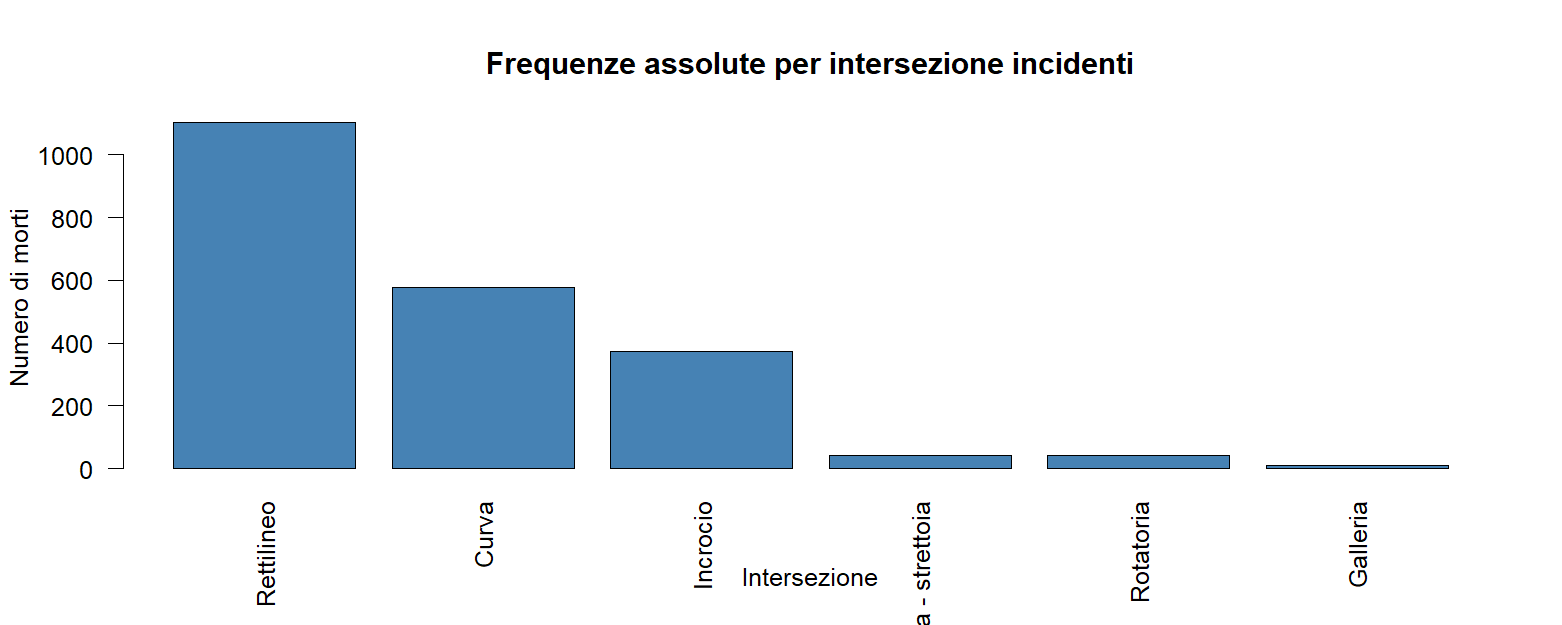
\includegraphics[width=13cm, height=7cm]{Rplot.png} % Adatta l'immagine alla larghezza del testo
\end{figure}

\begin{center}
\begin{lstlisting}[breaklines=true]
# Converti TIME_PERIOD in fattore per mantenere l'ordine originale
dati$TIME_PERIOD <- factor(dati$TIME_PERIOD, levels = unique(dati$TIME_PERIOD))

# Calcola il numero totale di morti per anno
morti_per_anno <- dati %>%
  group_by(TIME_PERIOD) %>%
  summarise(Totale_Morti = sum(Osservazione, na.rm = TRUE))

# Crea il grafico a linee con tutti gli anni visibili
ggplot(morti_per_anno, aes(x = TIME_PERIOD, y = Totale_Morti, group = 1)) +
  geom_line(color = "steelblue", size = 1) +
  geom_point(color = "steelblue", size = 2) +
  labs(title = "Andamento del numero di morti per incidenti stradali",
       x = "Anno",
       y = "Numero di morti") +
  theme_minimal() +
  theme(plot.title = element_text(hjust = 0.5),
        axis.text.x = element_text(angle = 45, hjust = 1, size = 8)) +  # Riduci dimensione testo
  scale_x_discrete(breaks = levels(morti_per_anno$TIME_PERIOD))  # Mostra tutti i valori
\end{lstlisting}  
\end{center}

\begin{figure}[H] % H forza la posizione esatta
    \centering
    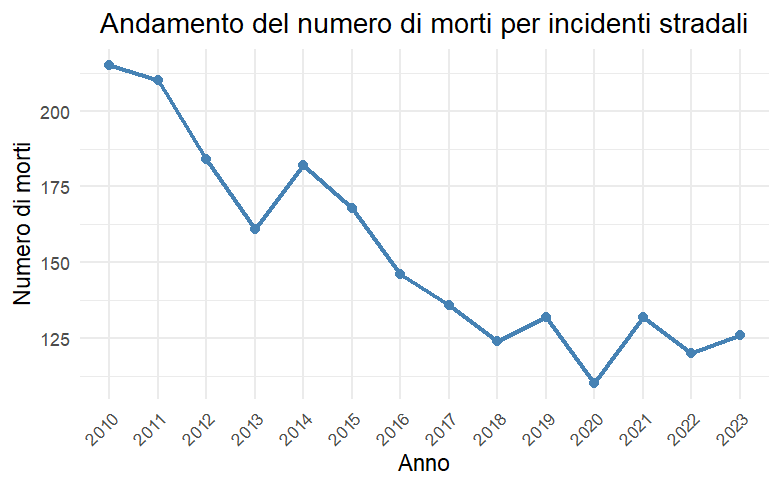
\includegraphics[width=12cm, height=7cm]{Rplot01.png} % Adatta l'immagine alla larghezza del testo
\end{figure}



\chapter{Indici di posizione}

\section{Media campionaria}
\begin{center}
\begin{lstlisting}[breaklines=true]
media_generale <- mean(dati$Osservazione, na.rm = TRUE)
print(paste("Media campionaria generale:", round(media_generale, 2)))
\end{lstlisting}  
\end{center}

\noindent
Output: "Media campionaria generale: 27.51"

\section{Mediana campionaria}
\begin{center}
\begin{lstlisting}[breaklines=true]
mediana_generale <- median(dati$Osservazione, na.rm = TRUE)
print(paste("Mediana generale:", mediana_generale))
\end{lstlisting}  
\end{center}
\noindent
Output: "Mediana generale: 15.5"


\section{Moda campionaria}

\chapter{Indici di variabilità} 

\section{Varianza campionaria}
    
\section{Deviazione standard campionaria}
    
\section{Scarto medio assoluto}

\section{Ampiezza del campo di variazione}

\section{Coefficiente di variazione}

\chapter{Indici di forma}
 
\section{Indice di asimmetria}

\section{Indice di curtosi} 



\end{document}